\documentclass[12pt, titlepage]{article}

\usepackage{booktabs}
\usepackage{tabularx}
\usepackage{hyperref}
\usepackage{graphicx}
\usepackage{float}



\hypersetup{
    colorlinks,
    citecolor=black,
    filecolor=black,
    linkcolor=red,
    urlcolor=blue
}
\usepackage[round]{natbib}

\title{SE 3XA3: Software Requirements Specification\\Title of Project}

\author{Team \#, Team Name
		\\ Student 1 Abdallah Taha and tahaa8
		\\ Student 2 name and macid
		\\ Student 3 name and macid
}

\date{\today}

\begin{document}

\maketitle

\pagenumbering{roman}
\tableofcontents
\listoftables
\listoffigures

\begin{table}[bp]
\caption{\bf Revision History}
\begin{tabularx}{\textwidth}{p{3cm}p{2cm}X}
\toprule {\bf Date} & {\bf Version} & {\bf Notes}\\
\midrule
Date 1 & 1.0 & Notes\\
Date 2 & 1.1 & Notes\\
\bottomrule
\end{tabularx}
\end{table}

\newpage

\pagenumbering{arabic}

This document describes the requirements for ....  The template for the Software
Requirements Specification (SRS) is a subset of the Volere
template~\citep{RobertsonAndRobertson2012}.  If you make further modifications
to the template, you should explicity state what modifications were made.

\section{Project Drivers}

\subsection{The Purpose of the Project}

\subsection{The Stakeholders}

\subsubsection{The Client}

\subsubsection{The Customers}

\subsubsection{Other Stakeholders}

\subsection{Mandated Constraints}

\subsection{Naming Conventions and Terminology}

\subsection{Relevant Facts and Assumptions}

User characteristics should go under assumptions.

\section{Functional Requirements}

\subsection{The Scope of the Work and the Product}

\subsubsection{The Context of the Work}
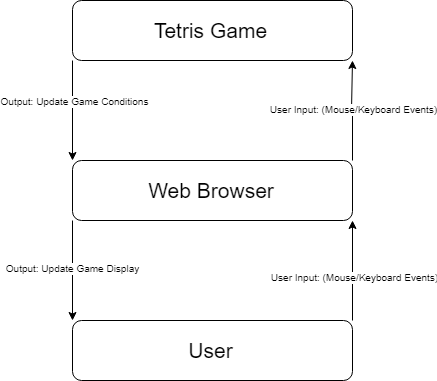
\includegraphics[width=0.95\linewidth]{Context.png}


\subsubsection*{Work Partitioning}
\begin{table}[H]
\caption{Work Partitioning Part I}
\begin{center}
\begin{tabular}{|c|c|c|c|}
\hline
Event Number & Event Name & Input & Output\\
\hline
1 & Tetris game Creation & Developer code & Web Browser\\
\hline
2 & Tetris game Audio & Microphone & Audio output device\\
\hline
3 & Tetris Full Row of Blocks & Developer graphics and code & Web Browser\\
\hline
4 & Blocks Overflow Outside of Grid & Developer code & Web Browser\\
\hline
5 & Tetris Score Calculation & Developer code & Web Browser\\
\hline
6 & Tetris Game Final Revision & Developer code & Web Browser\\
\hline
\end{tabular}
\end{center}
\label{default}
\end{table}%

\begin{table}[H]
\caption{Work Partitioning Part II}
\begin{center}
\begin{tabular}{|c|c|}

\hline
Event Number & Summary of BUC\\
\hline
1 & Recreate a terminal based game that works on multiple web browsers\\ 
\hline
2 & Record sound effect to be displayed in the game\\
\hline
3 & Create different functions to perform the game mechanics in this project\\
\hline
4 & Create overflow detection when blocks fall outside of grid then display an end screen\\
\hline
5 & Create a detection system for when row is full and calculate current score\\
\hline
6 & Finishing edits to the project\\
\hline

\end{tabular}
\end{center}
\label{default}
\end{table}%


    
    
\subsubsection{Individual Product Use Cases}

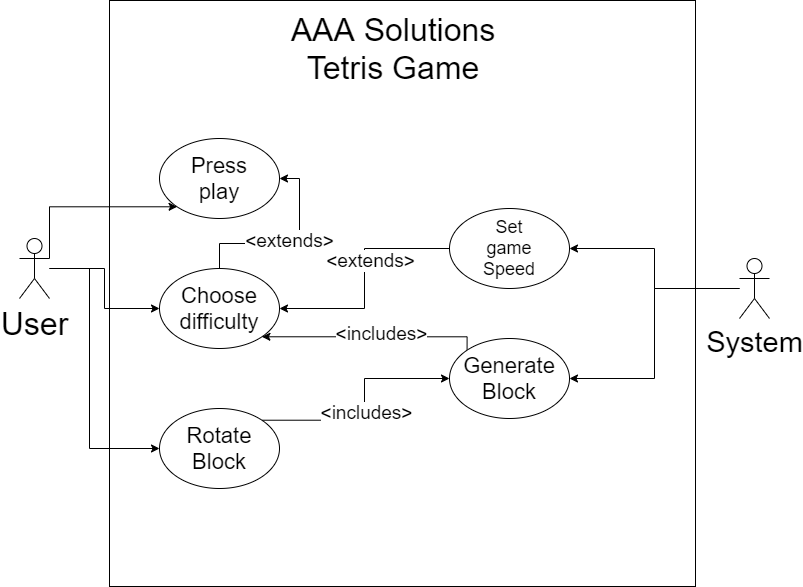
\includegraphics[width=0.95\linewidth]{usecasexa3.png}

\subsection{Functional Requirements}

\section{Non-functional Requirements}

\subsection{Look and Feel Requirements}

\subsection{Usability and Humanity Requirements}

\subsection{Performance Requirements}

\subsection{Operational and Environmental Requirements}

\subsection{Maintainability and Support Requirements}

\subsection{Security Requirements}

\subsection{Cultural Requirements}

\subsection{Legal Requirements}

\subsection{Health and Safety Requirements}

This section is not in the original Volere template, but health and safety are
issues that should be considered for every engineering project.

\section{Project Issues}

\subsection{Open Issues}

\subsection{Off-the-Shelf Solutions}

\subsection{New Problems}

\subsection{Tasks}

\subsection{Migration to the New Product}

\subsection{Risks}

\subsection{Costs}

\subsection{User Documentation and Training}

\subsection{Waiting Room}

\subsection{Ideas for Solutions}

\bibliographystyle{plainnat}

\bibliography{SRS}

\newpage

\section{Appendix}

This section has been added to the Volere template.  This is where you can place
additional information.

\subsection{Symbolic Parameters}

The definition of the requirements will likely call for SYMBOLIC\_CONSTANTS.
Their values are defined in this section for easy maintenance.


\end{document}